\documentclass[tikz,border=5pt]{standalone}
\usepackage[UTF8]{ctex}
\usepackage{amsmath,amssymb}
\usetikzlibrary{arrows.meta,calc,angles,quotes}
\definecolor{ink}{HTML}{243447}
\definecolor{blue}{HTML}{2765A2}
\definecolor{green}{HTML}{3F7D5B}
\definecolor{red}{HTML}{B74739}
\tikzset{body/.style={draw=ink,thick},vec/.style={draw=blue,thick,-{Latex}},
guide/.style={gray!60,dashed},dim/.style={ink,{Latex}-{Latex}},
line cap=round,line join=round}
\begin{document}
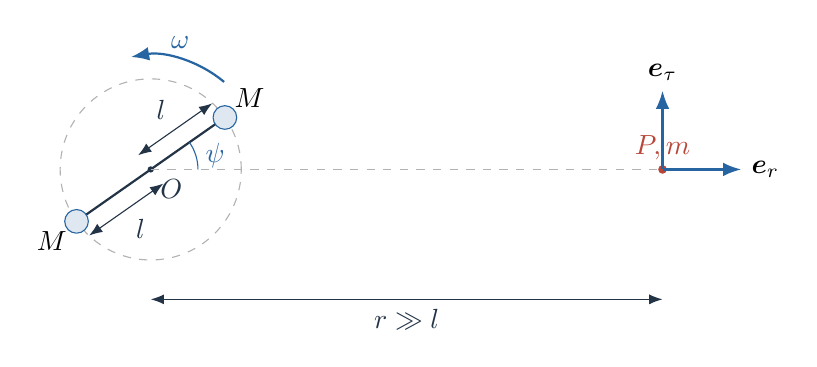
\begin{tikzpicture}
\coordinate(O)at(0,0);\coordinate(S)at(35:1.15);\coordinate(N)at(215:1.15);
\coordinate(P)at(6.5,0);
\draw[guide](O)circle(1.15);
\draw[body](N)--(S);
\filldraw[fill=blue!15,draw=blue](S)circle(.15)node[above right]{$M$};
\filldraw[fill=blue!15,draw=blue](N)circle(.15)node[below left]{$M$};
\fill[ink](O)circle(.04)node[below right]{$O$};
\fill[red](P)circle(.055)node[above]{$P,m$};
\draw[guide](O)--(P);
\draw[dim](0,-1.65)--(6.5,-1.65)node[midway,below]{$r\gg l$};
\draw[dim](-.16,.18)--($(S)+(-.16,.18)$)node[midway,above left]{$l$};
\draw[dim](.16,-.18)--($(N)+(.16,-.18)$)node[midway,below right]{$l$};
\draw[vec](P)--++(1,0)node[right]{$\boldsymbol e_r$};
\draw[vec](P)--++(0,1)node[above]{$\boldsymbol e_\tau$};
\draw[blue,-{Latex},thick](50:1.45)arc(50:100:1.45)node[midway,above]{$\omega$};
\draw[blue](.6,0)arc(0:35:.6)node[midway,right]{$\psi$};
\end{tikzpicture}
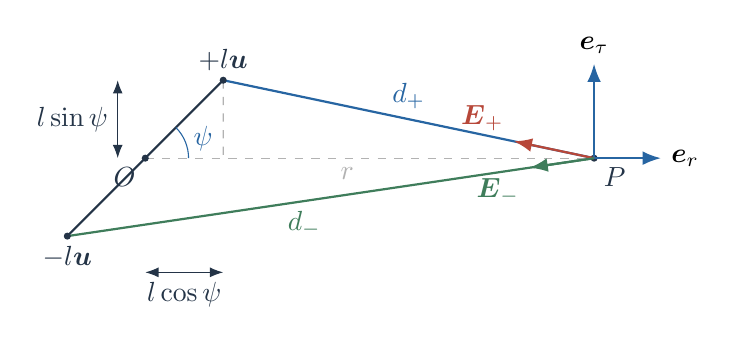
\begin{tikzpicture}
\coordinate(O)at(0,0);\coordinate(S)at(45:1.4);\coordinate(N)at(225:1.4);
\coordinate(P)at(5.7,0);
\draw[body](N)--(S);
\draw[blue,thick](S)--(P)node[midway,above]{$d_+$};
\draw[green,thick](N)--(P)node[pos=.45,below]{$d_-$};
\draw[guide](O)--(P)node[pos=.45,below]{$r$};
\draw[guide](S)--(.99,0);
\draw[dim](0,-1.45)--(.99,-1.45)node[midway,below]{$l\cos\psi$};
\draw[dim](-.35,0)--(-.35,.99)node[midway,left]{$l\sin\psi$};
\draw[blue](.55,0)arc(0:45:.55)node[pos=.6,right]{$\psi$};
\foreach\A/\pos in{O/below left,P/below right}
\fill[ink](\A)circle(.045)node[\pos]{$\A$};
\fill[ink](S)circle(.045)node[above]{$+l\boldsymbol u$};
\fill[ink](N)circle(.045)node[below]{$-l\boldsymbol u$};
\draw[vec](P)--++(.85,0)node[right]{$\boldsymbol e_r$};
\draw[vec](P)--++(0,1.2)node[above]{$\boldsymbol e_\tau$};
\draw[red,-{Latex},thick](P)--++(-1.02,.215)node[above left]{$\boldsymbol E_+$};
\draw[green,-{Latex},thick](P)--++(-.82,-.122)node[below left]{$\boldsymbol E_-$};
\end{tikzpicture}
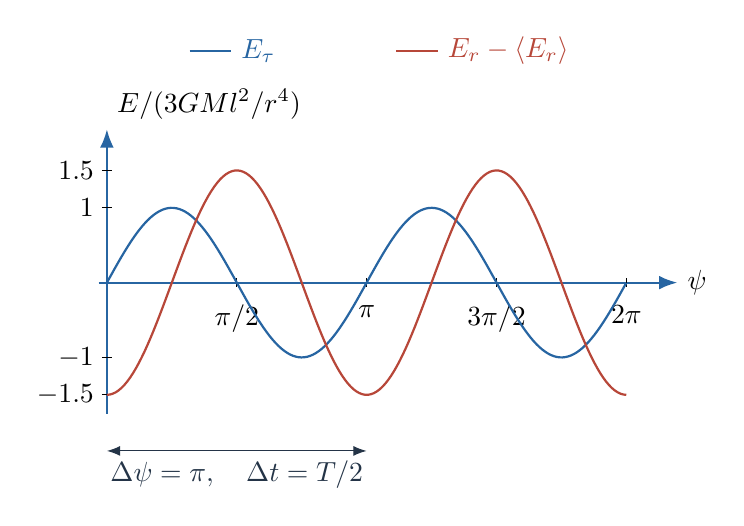
\begin{tikzpicture}[x=1.05cm,y=.95cm]
\draw[vec](-.1,0)--(6.9,0)node[right]{$\psi$};
\draw[vec](0,-1.75)--(0,2.05)node[above right]{$E/(3GMl^2/r^4)$};
\foreach\x/\lab in{1.5708/{\pi/2},3.1416/{\pi},4.7124/{3\pi/2},6.2832/{2\pi}}
\draw(\x,.06)--(\x,-.06)node[below=3pt]{$\lab$};
\foreach\y in{-1.5,-1,1,1.5}\draw(-.06,\y)--(.06,\y)node[left=3pt]{$\y$};
\draw[blue,thick,domain=0:6.2832,samples=180]plot(\x,{sin(2*\x r)});
\draw[red,thick,domain=0:6.2832,samples=180]plot(\x,{-1.5*cos(2*\x r)});
\draw[blue,thick](1,3.1)--(1.5,3.1)node[right]{$E_\tau$};
\draw[red,thick](3.5,3.1)--(4,3.1)node[right]{$E_r-\langle E_r\rangle$};
\draw[dim](0,-2.25)--(3.1416,-2.25)node[midway,below]{$\Delta\psi=\pi,\quad\Delta t=T/2$};
\end{tikzpicture}
\begin{tikzpicture}
\foreach\x/\angle/\time in{0/25/t,4.1/205/{t+T/2}}{
\begin{scope}[shift={(\x,0)}]
\draw[guide](0,0)circle(1.2);
\coordinate(A)at(\angle:1.2);\coordinate(B)at({\angle+180}:1.2);
\draw[body](A)--(B);
\filldraw[fill=blue!15,draw=blue](A)circle(.15)node[above]{$M$};
\filldraw[fill=green!15,draw=green](B)circle(.15)node[below]{$M$};
\fill[ink](0,0)circle(.03)node[below]{$O$};
\node at(0,-1.8){$\time$};
\end{scope}}
\draw[vec](1.7,.15)--(2.5,.15)node[midway,above]{半周};
\node[align=center]at(2.05,-2.5){颜色用于追踪两颗星体\\等质量交换后，引力源分布不变};
\end{tikzpicture}
\end{document}
